\colorlet{biologie}{andere}
\colorlet{physik}{andere}
\DTLsetpiesegmentcolor{1}{info}
\DTLsetpiesegmentcolor{2}{mathe}
\DTLsetpiesegmentcolor{3}{medizininfo}
\DTLsetpiesegmentcolor{4}{andere}
\DTLsetpiesegmentcolor{5}{sq}

\begin{Huge}
    Medizininformatik
\end{Huge}

\begin{exampleblock}{\textcolor{white}{Was ist der Studiengang?}}
    Die Schnittstelle zwischen Klinikum, Ärzten und Medizintechnikern. Klassische Anwendungsbereiche sind E-Health, Medizinische Datenverarbeitung sowie die (Mit-)Entwicklung von Medizingeräten. Es wird ein stärkerer Fokus auf Biologie, Physik und medizinische Inhalte gelegt. Ein Schwerpunktfach gibt es nicht. Danach kann das Studium mit einem Master \\ (4 Semester Regelstudienzeit) weitergeführt werden.
\end{exampleblock}

\begin{block}{Welcher Teil macht wie viel im Studium aus?}
    \begin{figure}[h!]
        \vspace{-20pt}
        \begin{minipage}{\linewidth}
            \centering
            \DTLloaddb{LPverteilungMedizin}{inhalte/medizininfo.csv}
            \tikzstyle{every node}=[text width={},minimum height=0pt]
            \DTLpiechart{
                variable=\lp,
                innerlabel={\parbox{40pt}{\centering\color{white} \bereich}},
                innerratio=0.25,
                radius=70pt,
                rotateinner}{LPverteilungMedizin}{\bereich=Bereich,\lp=LP}
        \end{minipage}
        \vspace{-20pt}
        \caption{Verteilung der Themenbereiche über das komplette Studium}
    \end{figure}
\end{block}

\begin{block}{Was macht man in welchem Semester?}
    \begin{figure}[h!]
        % 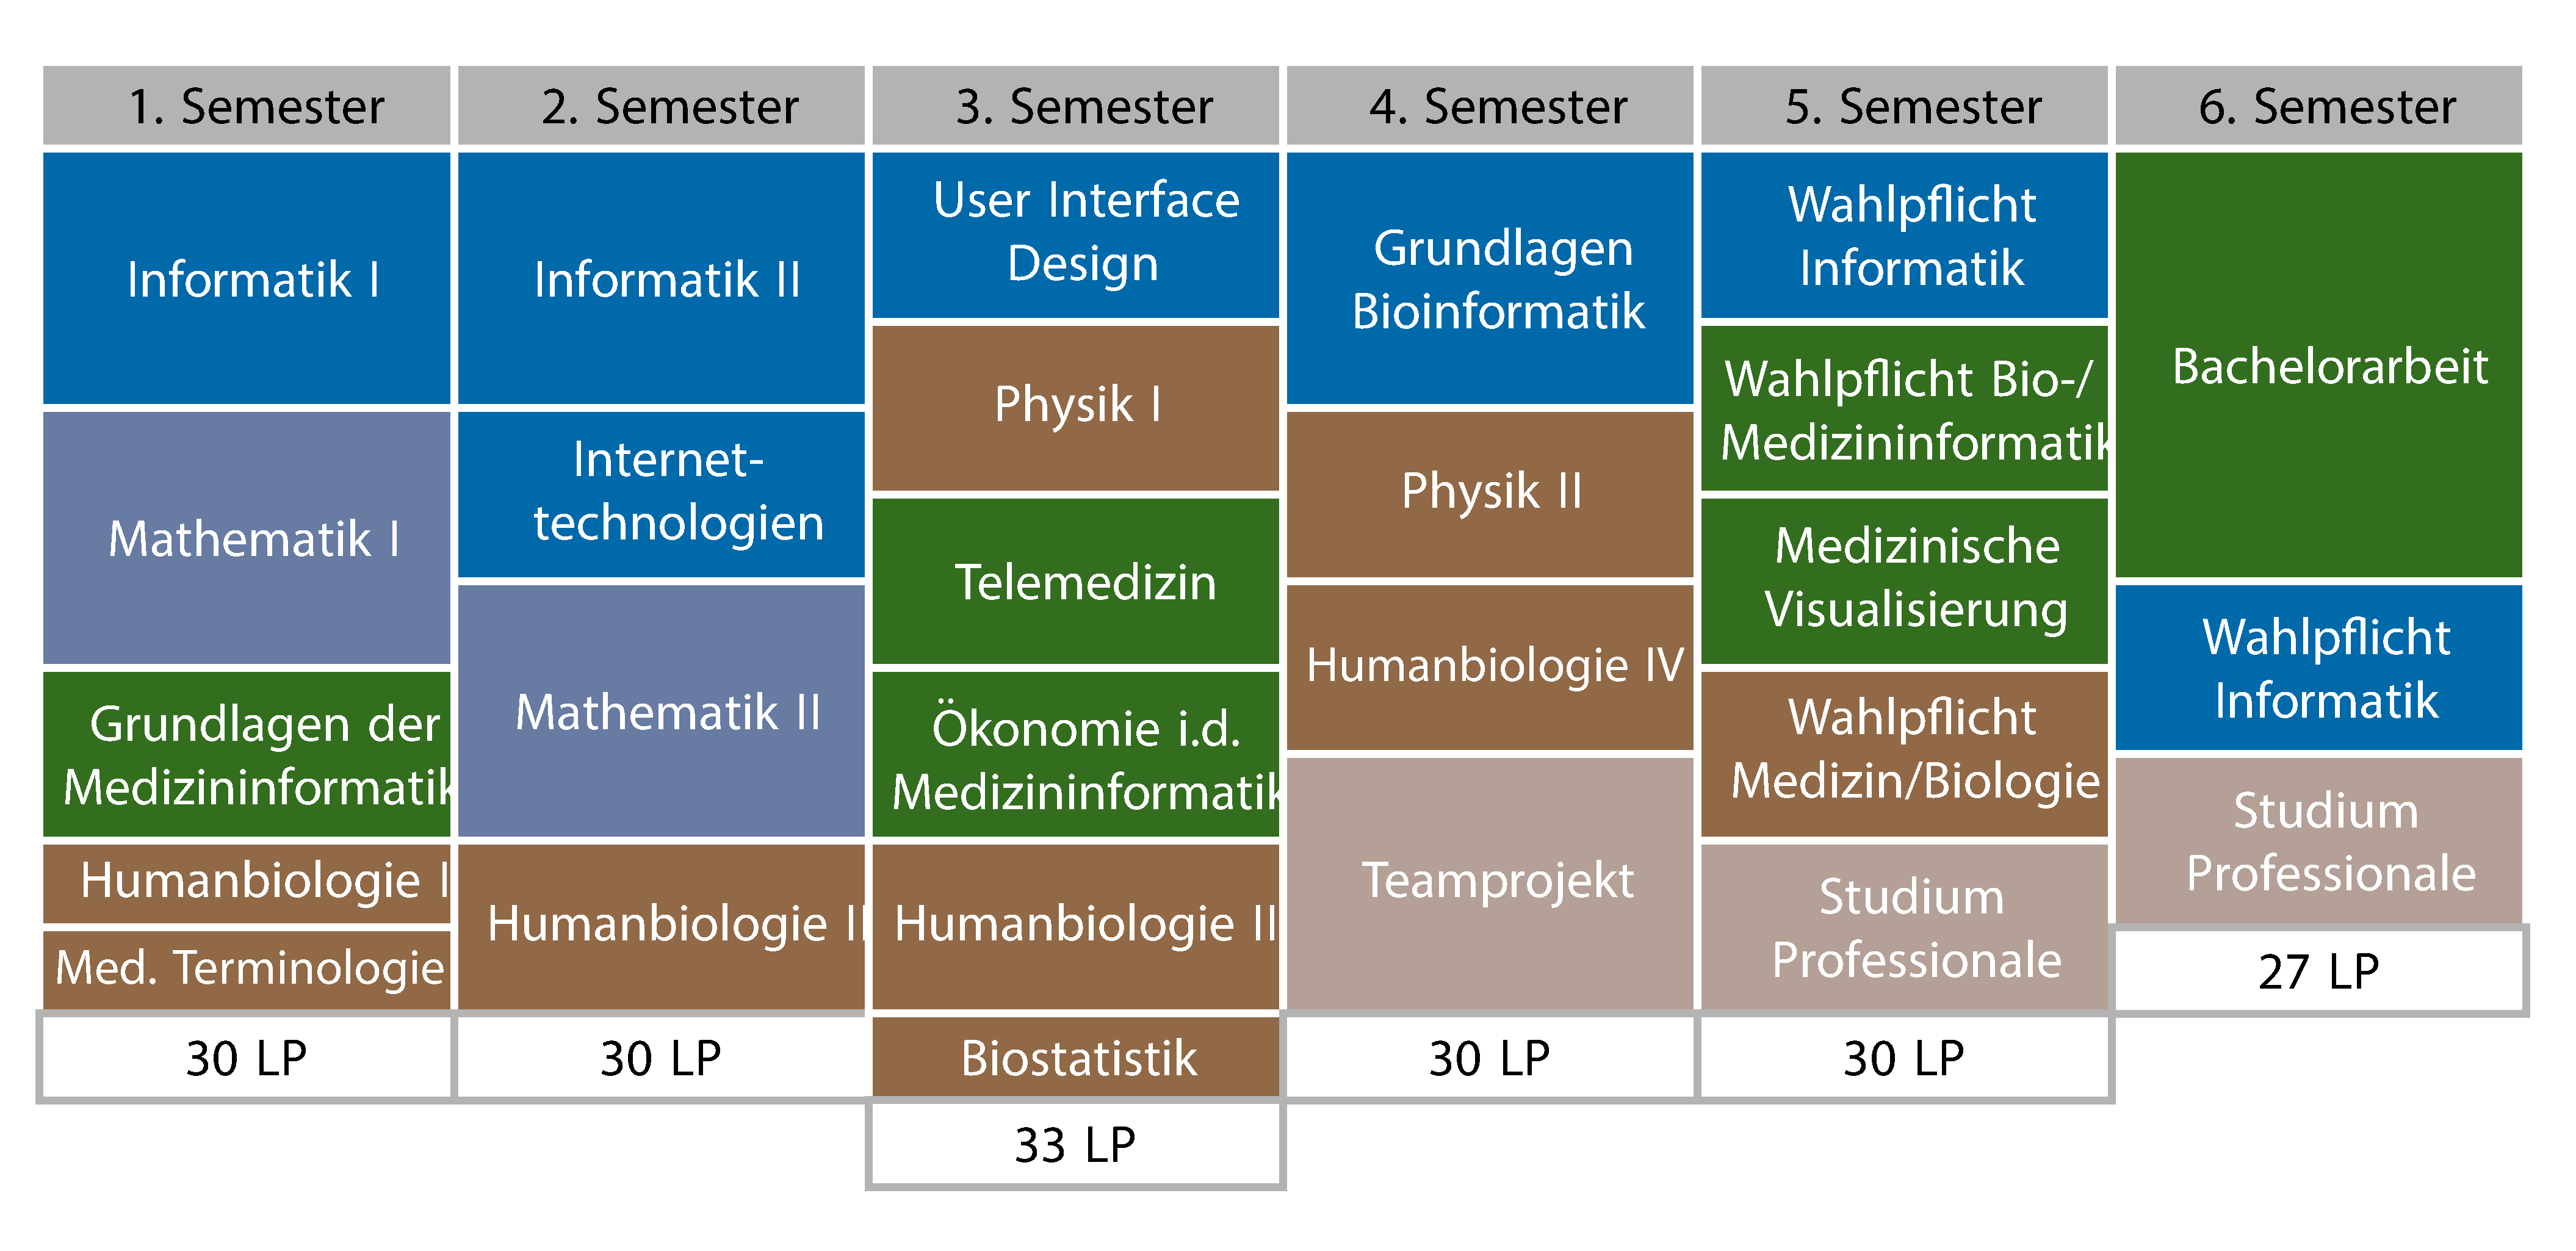
\includegraphics[width=\textwidth]{charts/medizininformatik_Studienplan_abWS18.pdf}
        % \includegraphics[width=\textwidth]{new/medizin_table.png}
        \resizebox{\linewidth}{!}{
        \begin{minipage}{\textwidth}
            \small
            \begin{tikzpicture}
                \begin{scope}[start chain=going below,node distance=\nodedistancecorrection]
                    \semester{1}
                    \veranstaltung{9}{Praktische In\-for\-ma\-tik~1}{info}
                    \veranstaltung{9}{Mathe\-matik f. Informatik~1}{mathe}
                    \veranstaltung{6}{Grundlagen der Medizininformatik}{medizininfo}
                    \veranstaltung{3}{Humanbiologie I}{biologie}
                    \veranstaltung{3}{Med. Terminologie}{biologie}
                    \SumLP{30}
                \end{scope}
                \begin{scope}[xshift=1\lpwidth,start chain=going below,node distance=\nodedistancecorrection]
                    \semester{2}
                    \veranstaltung{9}{Praktische In\-for\-ma\-tik~2}{info}
                    \veranstaltung{6}{Einf. Internet\-technologien}{info}
                    \veranstaltung{9}{Mathe\-matik f. Informatik~2}{mathe}
                    \veranstaltung{6}{Humanbiologie II}{biologie}
                    \SumLP{30}
                \end{scope}
                \begin{scope}[xshift=2\lpwidth,start chain=going below,node distance=\nodedistancecorrection]
                    \semester{3}
                    \veranstaltung{6}{User Experience}{info}
                    \veranstaltung{6}{Praktische Informatik 3}{info}
                    \veranstaltung{6}{Physik I}{physik}
                    \veranstaltung{6}{Humanbiologie III}{biologie}                
                    \veranstaltung{3}{Biostatistik}{biologie}                
                    \veranstaltung{3}{Ethik (übK)}{sq}
                    \SumLP{30}
                \end{scope}
                \begin{scope}[xshift=3\lpwidth,start chain=going below,node distance=\nodedistancecorrection]
                    \semester{4}                
                    \veranstaltung{9}{Grundlagen Bioinformatik}{medizininfo}
                    \veranstaltung{6}{Physik II}{physik}                
                    \veranstaltung{6}{Humanbiologie IV}{biologie}
                    \veranstaltung{9}{Team\-projekt}{sq}                
                    \SumLP{30}
                \end{scope}
                \begin{scope}[xshift=4\lpwidth,start chain=going below,node distance=\nodedistancecorrection]
                    \semester{5}
                    \veranstaltung{6}{WP Informatik}{info}
                    \veranstaltung{6}{Medizinische Visualisierung}{medizininfo}
                    \veranstaltung{6}{Telemedizin}{medizininfo}
                    \veranstaltung{6}{WP Medizin/Biologie}{biologie}
                    \veranstaltung{3}{Proseminar}{sq}
                    \veranstaltung{3}{übK}{sq}
                    \SumLP{30}
                \end{scope}
                \begin{scope}[xshift=5\lpwidth,start chain=going below,node distance=\nodedistancecorrection]
                    \semester{6}
                    \veranstaltung{6}{WP Bioinformatik}{medizininfo}
                    \veranstaltung{6}{WP Medizininformatik}{medizininfo}
                    \veranstaltung{15}{Bachelor\-arbeit}{medizininfo}
                    \veranstaltung{3}{übK}{sq}
                    \SumLP{30}
                \end{scope}
            \end{tikzpicture}
        \end{minipage}}
    \end{figure}
    
    Das 1. Semester ist nach Plan ein Wintersemester, der Studienbeginn ist hier auch nur zum Wintersemester möglich. 
    Dieser Verlauf ist lediglich ein Vorschlag und kein bindender Studienplan. Es empfiehlt sich jedoch, den Plan einzuhalten, wenn man in Regelstudienzeit studieren möchte.
\end{block}

\vfill
\begin{flushright}
    
\includegraphics[width=0.4\textwidth]{images/fsilogo.pdf}
\end{flushright}